\documentclass[12pt,a4paper]{article}
\usepackage{times}
\usepackage{durhampaper}
\usepackage{harvard}
\usepackage{listings}
\usepackage{color}
\definecolor{lightgray}{gray}{0.9}

\lstset{
    showstringspaces=false,
    basicstyle=\ttfamily,
    keywordstyle=\color{blue},
    commentstyle=\color[grey]{0.6},
    stringstyle=\color[RGB]{255,150,75}
}

\newcommand{\inlinecode}[2]{\colorbox{white}{\fontsize{10}{10}\lstinline[language=#1]$#2$}}

% ---------------------------------
% ---- PACKAGES -------------------
    % package to add wrap figure
    \usepackage{wrapfig}
    % packages to add images
    \usepackage{graphicx}
    % packages for pseudo-code and algorithms
    \usepackage{amsmath}
    \usepackage{algorithm}
    \usepackage[noend]{algpseudocode}
    \makeatletter
    \def\BState{\State\hskip-\ALG@thistlm}
    \makeatother
    % packages to generate neural network graph
    \usepackage{tikz}
    \usetikzlibrary{matrix,chains,positioning,decorations.pathreplacing,arrows}
    % package to add graphs
    \usepackage{pgfplots}
    % stuff for checker board
    \usetikzlibrary{matrix.skeleton}
    \tikzstyle{ball} = [circle, shading=ball, minimum size=1cm]
    \newcommand{\bl}{\node [ball, ball color=black!80!white, draw=black!65!white, thin]{};}
    \newcommand{\wh}{\node [ball, ball color=white] {};}
    \pgfplotsset{compat=1.15}
% ---- END PACKAGES ---------------
% ---------------------------------

    \citationmode{abbr}
    \bibliographystyle{agsm}
    % Titular Information
    \title{A Neuroevolutionary Approach to Draughts Playing Agents}
    \author{}
    \student{T. P. Nguyen}
    \supervisor{S. Dantchev}
    \degree{BSc Computer Science}
    \date{}

    % Start the Document
    % Note that the whole report, including the references, should not be longer than 20 pages in length.  The system will not accept any report longer than 20 pages.  It should be noted that not all the details of the work carried out in the project can be represented in 20 pages.  It is therefore vital that the Project Log book be kept up to date as this will be used as supplementary material when the project paper is marked.  There should be between 10 and 20 referenced papers---references to Web based pages should be less than 10\%.
    \begin{document}
    \maketitle


\begin{abstract}
    % These instructions give you guidelines for preparing the final paper.  DO NOT change any settings, such as margins and font sizes.  Just use this as a template and modify the contents into your final paper.  Do not cite references in the abstract.

    % The abstract must be a Structured Abstract with the headings {\bf Context/Background}, {\bf Aims}, {\bf Method}, {\bf Results}, and {\bf Conclusions}.  This section should not be longer than half of a page, and having no more than one or two sentences under each heading is advised.

    {\bf Background}

    Presently, competitive Draughts AI players are designed to play at a fixed ability. While it has produced very competitive and intelligent players, they require some human intervention to improve their performance. 
    This is mainly due to their dependency on pre-defined move databases. Optimal moves are pre-calculated, and recalled when necessary. Through neuroevolution, this issue could be solved by creating a player that can grow in ability over time, by learning to play itself.
    
    {\bf Aims}

    The objective of this project is to explore how well a neuroevolutionary approach can tackle the game of English Draughts. First, previous historical successes in the field and the components that helped build their systems are studied. Then, the components are looked to see how they can be adapted to suit the objective at hand. 

    {\bf Method}

    % The initial population consists of randomly generated AI players, which will play each other to determine the best player out of the population. The performance of championing AI players at every generation of the genetic algorithm are measured against previous champions. Appropriate algorithms are implemented to determine the overall development of the system's ability to play Draughts.
    The method starts with designing a feed-forward neural network that takes as input, the state of a checker board, and outputs an evaluation of the players advantage. This is then used in a algorithm that evaluates future moves to predict the best move at a given position. This, alongside a set of weights for the neural network, creates a system that can evaluate potential moves. Finally, the system is used on an existing Draughts framework that will provide the player with the ability to play Draughts. Genetic algorithms are used to adjust the weights of the neural network, with the intention of making the system learn to evaluate checker boards more precisely. 
    
    {\bf Results}

    Overall, the neuroevolutionary approach has shown to learn and improve over time. The net learning rate was positive. However, the wide scope of the adjustments afforded may have impacted the learning rate and has consequently shown to be volatile in some situations. The use of crossovers may dramatically influence the quality of the learning.

    {\bf Conclusion}

    Under the premise that the fitness function is well defined, neuroevolution can be considered as an option to create a draughts playing AI. However, the robustness of the system is quite volatile. To counteract this, the system is  best paired with mutation and crossover methods that are not heavily reliant on entropy.

\end{abstract}
% Done
\begin{keywords}
    Artificial Intelligence, Machine Learning, Neural Networks, Neuroevolution, Genetic Algorithms, Draughts, Checkers, Crossover, Monte Carlo Tree Search
\end{keywords}
% DONE
\section{Introduction}
    % This section briefly introduces the general project background, the research question you are addressing, and the project objectives.  It should be between 2 to 3 pages in length.  Do not change the font sizes or line spacing in order to put in more text.
    The intention of this project is to explore the effectiveness of genetic algorithms to improve the neurons of a neural network. Neural networks can be used to evaluate the performance of two players in a zero-sum game of Draughts. We attempt to manipulate the neurons through the use of genetic algorithms to increase the accuracy of the evaluation. This would potentially allow us to create an effective Draughts playing agent that, when provided with the option to consider a set of moves, would have the ability to play and learn without human input.

    \subsection{Draughts}

    English Draughts (also known as American Checkers) is a popular 2-player board-game played on an 8x8 chess board (also known as a checker board/draughts board). Players choose a colour and begin with 12 pawns of their respective colours, which are placed on the dark-coloured squares of the board. Beginning with the black pawns, each player takes a turn to move a pawn diagonally in one square. In the event that a pawn reaches the opposite side of the board from where the piece originated, it is promoted to a king. Kings have the ability to traverse backwards in the same diagonal motion as pawns. Assuming that there is space upon landing, a piece (pawn or king) also has the option to capture their opponents piece by moving two consecutive diagonal squares, where the opponents piece is situated immediately opposing the players piece. Pieces can be captured consecutively in a single turn if the moves afford the scenario. A player wins by capturing all of their opponents pieces. A player loses by having all of their pieces captured. A draw occurs when both players agree to draw after a three-fold repetition (where both players take three moves to simulate the same position), or a player has pieces on the board but cannot move any of them. A draw can also be forced when both players fail to capture a piece after a set amount of moves.

    \subsection{Neural Networks}

    Neural Networks are non-linear statistical data-modelling tools which link inputs and outputs adaptively in a learning process similar to how the human brain operates. Networks consist of units, described as neurons, and are joined by a set of rules and weights. The neurons are defined with some characteristics and appear in layers. The first layer is defined as the input layer, and the last layer is the output. Layers between the two aforementioned are described as hidden layers. Data is analysed by their propagation through the layers of neurons, where each neuron manipulates the content of the data by some manner. Learning takes place in the form of manipulation on the weights connecting the neurons. This allows it to model complex relationships between inputs and output, and it can also find patterns in the data. 

 	\subsection{Genetic Algorithms}

    A subset of evolutionary algorithms in general, Genetic algorithms (GAs) are a group of search techniques used to find exact or approximate solutions to optimisation and search problems. The methodology is inspired by Charles Darwin's evolutionism theory; individuals are created based on the improvement of their ancestors genetic information (genome). Genomes are analogical to a data structure, most commonly a 1D array. Evolutionary algorithms typically consist of a population of agents, a tournament selection process, and the introduction of probabilistic mutation on genomes. This in turn allows evolutionary algorithms to create genomes that increase in quality over time in regards to the tournament. Genetic algorithms distinguish themselves from evolutionary algorithms through their use of algorithmic crossover mechanisms, where two parent genomes are combined together to create offspring. The use of evolutionary algorithms to train neural networks is described as a type of machine learning called Neuroevolution.

    \subsection{Aims}

    % Research Question
    Whilst the use of evolutionary algorithms and neural networks have been explored independently of one another to create draughts players, my intention is to explore the effectiveness of the combined methods in terms of developing an artificially intelligent draughts playing agent. 

    \subsubsection{Minimum Objective}
        % The minimum objective of this project was to design and build a programme that would display a polygonal mesh of triangles, with help of a mesh data structure. The basic mesh data structure would have to enable future features that the next objectives would require.
        The minimum objective is to implement a feed-forward neural network, alongside a Draughts game interface for the network to evaluate on. This will need to pair with a decision making algorithm that determines the move to choose at a given state of the game. Finally, a simple genetic algorithm would also need to be implemented that interacts with the neural network, allowing the possibility to learn over time.

    \subsubsection{Intermediate Objective}
        % The intermediate objective of this project was to create and incorporate the algorithms for the calculation of triangle surface normals, vertex normals and gradient (following our definition) in the initial programme, and enable visualisation of the “interesting” gradient changes and vertex normals on the mesh displayed by the programme.
        The intermediate objective involves the implementation of an interface to play against the trained result, and to create a monte-carlo tree search  algorithm. This would allow the system to think in ahead, allowing it to evaluate better quality decisions. Also, as the genetic algorithm includes a tournament mechanism which will play many games simultaneously, this will need to be implemented to run in parallel.
        
    \subsubsection{Advanced Objective}
        % The advanced objective of this project was to evaluate the speed of the algorithms and compare it to the time complexity that we obtained from theoretical analysis of the algorithms. The final sections of this paper will show the results acquired and the analysis and evaluation of the work we carried out. 
        The advanced objective consists of producing a system that indicates that it is learning over time. The later sections of this paper evaluates the quality of the learning rate and other results that determine the extent of its success.
    
    
    % To template the document, the remaining sections of the paper discusses related and relevant work, the proposed solution, results and an evaluation of the project. The paper is then wrapped up with a conclusion, discussing the implications of the project and potential future work.

% TODO
\section{Related Work}
    % This section presents a survey of existing work on the problems that this project addresses. it should be between 2 to 4 pages in length.  The rest of this section shows the formats of subsections as well as some general formatting information for tables, figures, references and equations.

    % Intro
        Although Draughts is a perfect information game, it was historically used as a testing ground for artificial intelligence and computational capabilities since the early introduction of computers. This was due to the relatively vast search space, making the game difficult to brute-force, until recently. Research has shown that it was possible in theory to solve the game, but the computational performance was not available to prove the method at the time of discovery \cite{schaeffer_solving_1996}. The same researchers however reinvestigated the research a decade later, eventually proving the game to be \emph{weakly-solved}. \cite{schaeffer_checkers_2007}. Weakly-solvable is defined such that ``the game-theoretic value for the initial position has been determined, and that a strategy exists for achieving the game-theoretic value from the opening position.'' \cite{allis_searching_1994} However, the premise of this paper was not necessarily to solve the game itself, but to rather see whether neuroevolution was a method that, when measured via its ability to play the game, shows that it can evolve in performance over time.

        Research in artificial intelligence alone has been active since, targeting games with a higher move space, notably Chess and, more recently, Go. This section will summarise specific and notable techniques relevant to the discussion of the task at hand.

    % DONE
    \subsection{Arthur Samuel}
        In 1959, An early design of machine learning to play Draughts was devised by Arthur Samuel\cite{samuel_studies_1959}. His algorithm was based on the continual improvement of a linear combination of heuristics, which act as an evaluator function for a given state of the checker board. The heuristics represented different strategies one would have considered when playing Draughts. Some of these heuristics include the number of pieces on side (such that one side was shown to have a particular advantage given that they have more pieces), and the number of pieces positioned along the central diagonal. His evolutionary strategy consisted of agents, each of which represented coefficient values for the heuristics (initially random), and new agents are formed via the manipulation of its successor's coefficients with subtle mutations.
        
        % The weights were then trained by the algorithm playing itself in a form of genetic programming. 
        
        % talk about minimax here.
        Samuel's decision making algorithm primarily revolved around an early concept of the mini-max algorithm. This algorithm takes as input the present state of the checker board, and returns the best move to choose. Mini-max algorithm can be described using the following instructions:
        
        \begin{enumerate}
            \item Each node represents a state of a checker board. Child nodes represent a future state of the checker board, given a move. Child nodes can only be produced from the parent node; i.e. a move from a parent node will produce a child node.
            \item Child nodes are expanded until some depth is reached. From here, an evaluation function is used to calculate the value of the leaf nodes at this depth. This evaluation function produces a value that indicates a players advantage in a given state.
            \item The best potential position for a given player can be deduced from the nodes at this stage, which is quantified with a value.
            \item The best value propagates upwards until it reaches to a child of the root node. This represents an agent's current state of the game.
        \end{enumerate}

        The use of alpha-beta pruning helped to ignore evaluating disadvantageous states, reducing the overall number of neural network evaluations. Once the possible moves have been considered, the best child node is chosen, representing the best move at a given position.
    
        There are inherent trade-offs to this decision algorithm, especially with utilising higher ply counts; asymptotic complexity of mini-max is exponential; it being $O(x^y)$ for $x$ being the branching factor, and $y$ being depth. The branching factor consists of the moves from each agent in a given game. This exponential growth is the achilles heel to the mini-max approach. 

        A later investigation by a checkers magazine evaluated Samuel's player to perform at below Class B \cite{schaeffer_one_1997,fogel_evolving_2000}; (Class B being categorised with an ELO range of [1600-1799]). This implied that it played at a performance that can be seen at club level players. However, the performance of the system is handicapped by the quality of the heuristics Samuel devised; i.e. the system can only be as good as whatever Samuel considered as a heuristic to consider when deciding what move to make.

    % DONE
    \subsection{Blondie24}
        The idea of evolving neural networks to evaluate board-states was based on the success Chellapilla and Fogel had in evolving their own Draughts playing neural networks. Their method used Samuel's system as a foundation and modified the evaluation method, using feed-forward neural networks instead of a distinct linear combination. Their resulting player, Blondie24, was then taught to play without priori knowledge in a similar vein to Samuel's system. \cite{chellapilla_evolving_1999}

        Blondie24 used an evolutionary algorithm, using a population of fifteen agents $i=1,\dots,15$, each of which consisted of two properties. The first property were weights of the neural network (which are initially random), with the second property being a self-adaptive parameter vector, $\tau_i$, which determined how random the mutations are when the agent $i$ evolved. 

        \begin{figure}[ht!]
            \centering
            \begin{equation}
            \tau_i(j) = \tau_i(j) \cdot e^{\mu}
            \end{equation}
            \caption{The mutation formula in Blondie24, where $j=1,...,N_w$ represents individual weight of the neural network $w$, and $\mu$ representing a random decimal in the range of $[0-1]$. \label{blondieMutation}}
        \end{figure}
        
        In each generation, every agent plays each other in a round robin style tournament. Agents plays an equal number of games, and successors are chosen based on their performance in the tournament. The best agents are chosen to mutate themselves, producing new agents in the chance that the new agents perform better than prior. Mutation was performed using the formula in Figure \ref{blondieMutation}. Like Samuel's program, Blondie24 also used Mini-Max with alpha-beta pruning.

        However, crossover mechanisms were not considered (and therefore cannot be classified as using genetic algorithms). Blondie24's neural network structure consists of a $\left\{ 32,40,10,1 \right\}$ set, such that the input layer consisted of 32 nodes, and 1 output node. The output node representing a classifier value in the range of [-1, 1], representing a particular advantage for a given side of the board. One issue with this particular method was that spatial awareness could not be immediately interpreted as it takes an immediate input of the positions on the board. This makes it inherently more difficult for the neural network to generate heuristics based on spatial awareness.

        We do not wish to repeat this work, but it is important to understand that we wish to abstract and modularise parts of the best features of this system to modify and extend them to the solution described in the paper.

    \subsection{Post Blondie24}

        Blondie24 was influential in the field of neuroevolution during its time, leading to various studies on the theory behind its success. A notable example was the series of publications by Al-Khateeb and Kendall, where they explore in detail the different features that comprise Blondie24. One of their studies concerning the effects of the the ply depth, concluded that having a higher ply-depth unsurprisingly increases the overall performance of the player, and that agents trained at a higher ply performs significantly worse when playing at a lower ply. More importantly, the results in the paper suggest that a 4ply depth produces the best value function to start with during the learning phase, and increasing the ply depth for evaluations. \cite{al-khateeb_effect_2012} Their study in the influence of tournaments in Blondie24 concluded that the league structure seemed more appropriate to use as opposed to the round robin tournament. \cite{al-khateeb_introducing_2009} This is however more difficult to set up in parallel, which may be a largely contributing factor during the implementation of the system.
        
        % Alternative contemporary machine learning techniques have been exercised against Draughts. Franken et al. (2003) used draughtsboards as an evaluator for their rendition of an AI through Particle Swarm Optimisations.[14] 
        % Within research in the game of Draughts alone, A research by Toledo-Marin et al. looked at studies on attacking strategies using Draughts as a reference (which however can be applied to any other zero-sum game), where they mathematically prove that for an offensive player, maximising the offensive improves their probability to win.\cite{toledo-marin_is_2016} This could be considered to guide the system to lean towards attacking moves, which could potentially accelerate the learning rate of the system.

        % Stanford's SVM method of improving Blondie
        % Cobbe, et al. improves Blondie24 by using an evaluation function that consists of Support Vector Machines, which achieves locally optimal performance in approximately a third as many generations than its typical evolution. \cite{cobbe_accelerating_nodate} 
        
    % TODO: fix write up of everything, talk about monte-carlo
    % \subsection{Neural Networks}
    %     % need to mention regular gradient based learning
    %     Lai's Giraffe \cite{lai_giraffe:_2015} program used a deep reinforcement learning technique to play Chess to an advanced level in a relatively quick time-period. Giraffe's decision function involved using Temporal Difference Learning (TD-Leaf), an improvement on MiniMax, by Baxter et al. \cite{baxter_tdleaflambda_1999} However, Giraffe has been trained on previously played games from grandmaster tournaments as a reference, and was not entirely self-taught.
        % Lai then moved on to join DeepMind, 

        % talk about monte-carlo

    % TODO: fix writeup of everything
    \subsection{Return of Genetic Algorithms}

        Since then, there has been a non-trivial number of published papers describing the promising utility of genetic algorithms and neural networks in general. Genetic algorithms have been shown to evolve weights for a convolutional neural network in a classification task better than back-propagation, in nearly all situations, other than when the number of generations generated for neural networks are small. \cite{perez_apply_nodate} Another research showed its ability to compute optimal structures for deep neural networks, using an image recognition dataset as the benchmark for competitiveness against the networks. \cite{xie_genetic_2017}
        
        % Kusiak et al. (2007) have devised the use of pure genetic algorithms as the premise to evaluate the board. [16] they describe the use of 25 heuristics that, when used in unison, can determine the evaluation of a given board. They continue to go further on and specify that various combinations of heuristics, when used in different stages of the game, prove to be the most promising of outcomes.

        % Uber's revival of genetic algorithms and safe mutations
        However, one recent paper by Clune et al. on behalf of Uber Labs returned to the use of genetic algorithms as a basis to train especially deep convolutional networks with success. \cite{such_deep_2017} Their neuroevolutionary system was used to play popular Atari games on the OpenAI frame  work, and was found to perform as well as other contemporary evolution strategies and reinforcement learning algorithms. 

        The success of the program was based on their system's ability to perform safe mutations, a technique that revolves around measuring the sensitivity of the network to changes with some of the weights. \cite{lehman_safe_2017} This afforded the system to evolve deep neural networks (In this particular case, containing over 100 layers and over four million weights and biases,) in a manner that allowed random but safe and exploratory searches. Their safe mutation exploits the knowledge of the neural network structure, by retaining sampled experiences of the network (inputs that feed into the network and its outputs). This allows the weights to be manipulated by comparing its significance with the output, by comparing it with the sampled experiences. 

        However, they also do not consider the use of crossover techniques in their paper, but they briefly mention that it would very well be possible to produce a safe crossover method that exploits structures of a neural network, inspired by their research produced on safe mutations.

        Unfortunately, it was unrealistic to apply the same techniques described in their paper into the proposed system. The machine used as the base (consisting of hundreds to thousands of cores) was of a magnitude greater than what was available for the task at hand, but a more simplistic and adapted model can be produced using similar ideas. 
        
        A popular trend between the contemporary research was the shared absence of the use of crossover algorithms. One paper describes the use of different crossover algorithms on neural networks having no clear advantage over each other, in comparison to a uniform crossover (uniform crossovers are also commonly defined as the textbook crossover) which disrupted the overall performance of the neural networks. This could be due to building blocks being disrupted as chunks of the sequential weights are swapped out of each other \cite{emmanouilidis_comparison_2000}. It was important to consider this when devising a crossover method, such that the effect it has on the neural network should be subtle enough that it should pose similar results to the network prior to crossovers.

% TODO: Write up everything..
\section{Solution}

    % This section presents the solutions to the problems in detail.  The design and implementation details should all be placed in this section.  You may create a number of subsections, each focussing on one issue.  

    % This section should be between 4 to 7 pages in length.
        
    This section describes the implementation process of the system. Implementing the checker board interface is not included in the discussion as it is not one of our objectives. However, the sections below are considered under the premise that the interface was built prior to their development.

    \subsection{Evaluation Function}
        % Neural Net figure
        \begin{figure}[ht!]
            \centering
            \caption{The chosen neural network model. The preprocessed values of the checker board are used as input. An output was produced after propagation that ranged from [-1,1]. \label{nnmodel}}
            \vspace{10pt}
            \tikzset{%
                every neuron/.style={
                    circle,
                    draw,
                    minimum size=0.6cm
                    },
                neuron missing/.style={
                    draw=none, 
                    scale=4,
                    text height=0.2cm,
                    execute at begin node=\color{black}$\vdots$
                },
            }

            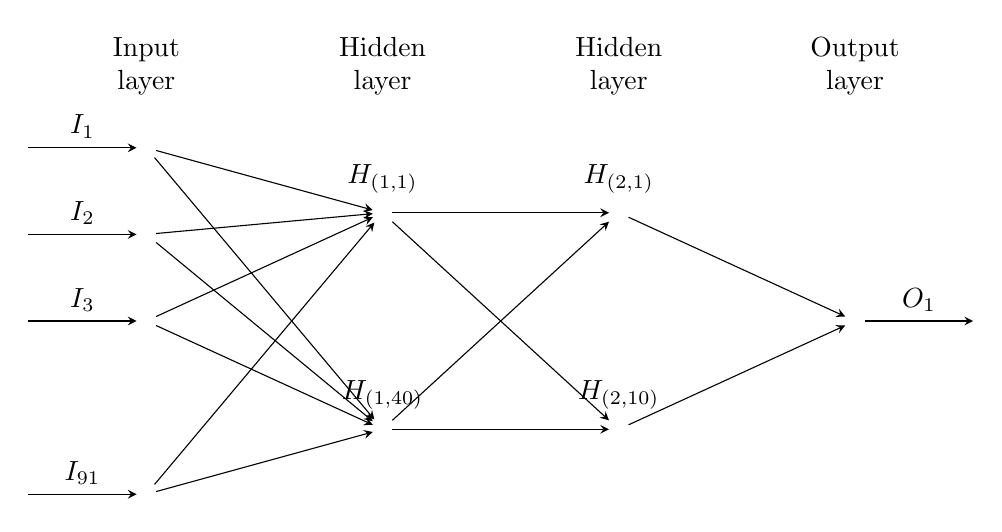
\begin{tikzpicture}[x=1.5cm, y=1.1cm, >=stealth]

                % draw nodes
                    % % input values
                    % \foreach \m/\l [count=\y] in {1,2,3,missing,4}
                    % 	\node [every neuron/.try, neuron \m/.try] (input-\m) at (-0.5,2.5-\y) {};

                    % input layer
                    \foreach \m/\l [count=\y] in {1,2,3,missing,4}
                    \node [every neuron/.try, neuron \m/.try] (input-\m) at (0,2.5-\y) {};
                    
                    % layer 1
                    \foreach \m [count=\y] in {1,missing,2}
                    \node [every neuron/.try, neuron \m/.try ] (hidden1-\m) at (2,2-\y*1.25) {};

                    % layer 2
                    \foreach \m [count=\y] in {1,missing,2}
                    \node [every neuron/.try, neuron \m/.try ] (hidden2-\m) at (4,2-\y*1.25) {};

                    % output layer
                    \foreach \m [count=\y] in {1}
                    \node [every neuron/.try, neuron \m/.try ] (output-\m) at (6,0.5-\y) {};

                % input layer
                \foreach \l [count=\i] in {1,2,3,91}
                    \draw [<-] (input-\i) -- ++(-1,0)
                    node [above, midway] {$I_{\l}$};

                % hidden 1
                \foreach \l [count=\i] in {{(1,1)},{(1,40)}}
                    \node [above] at (hidden1-\i.north) {$H_{\l}$};

                % hidden 2
                \foreach \l [count=\i] in {(2,1),(2,10)}
                    \node [above] at (hidden2-\i.north) {$H_{\l}$};

                % output layer
                \foreach \l [count=\i] in {1}
                    \draw [->] (output-\i) -- ++(1,0)
                    node [above, midway] {$O_\l$};

                % lines from input to hidden 1
                \foreach \i in {1,...,4}
                    \foreach \j in {1,...,2}
                        \draw [->] (input-\i) -- (hidden1-\j);
                
                % lines from hidden 1 to hidden 2
                \foreach \i in {1,...,2}
                \foreach \j in {1,...,2}
                    \draw [->] (hidden1-\i) -- (hidden2-\j);

                % lines from hidden 2 to output
                \foreach \i in {1,...,2}
                    \foreach \j in {1}
                        \draw [->] (hidden2-\i) -- (output-\j);

                % headings
                \foreach \l [count=\x from 0] in {Input, Hidden, Hidden, Output}
                    \node [align=center, above] at (\x*2,2) {\l \\ layer};

            \end{tikzpicture}
            % \vspace{-25pt}
        \end{figure}
        
        % \begin{wrapfigure}{r}{0.37 \textwidth}
            %     % \begin{center}
            %     \fontsize{8}{11}
            %     % \vspace{-40pt}
            %     \centering
            %         \caption{The indexes of the 32 pieces of the input layer are the immediate values of the positions on the board. \label{boardarray}}
            %         \vspace{5pt}
            %         \begin{tikzpicture}
            %         \color{white}
            %         \matrix (m) [matrix of nodes, nodes in empty cells, label skeleton, nodes={minimum size = 0.4cm}] {
            %         & 31 &&30&&29&&28 \\
            %         27 &&26&&25&&24&&\\
            %         &23&&22&&21&&20\\   
            %             19&&18&&17&&16&&\\
            %         &15&&14&&13&&12\\
            %         11&&10&&9&&8&&\\
            %         &7&&6&&5&&4\\
            %         3&&2&&1&&0\\
            %         % \bl &     & \bl &     &     &     & \bl &     \\
            %         %     &     &     & \bl &     &     &     &     \\
            %         % \wh &     &     &     &     &     &     &     \\
            %         %     &     &     & \wh &     & \wh &     & \wh \\
            %         % \wh &     & \wh &     & \wh &     & \wh &     \\
            %         %     & \wh &     & \wh &     & \wh &     & \wh \\
            %         };
            %         \foreach \row in {1, ..., 8} {
            %         \foreach \col in {1, ..., 8} {
            %             \pgfmathparse{Mod(\row + \col, 2) ? "black" : "white"}
            %             \colorlet{squarebg}{\pgfmathresult}
            %             \fitandstyle[background]{(m-cell-\row-\col)}{fill = squarebg}
            %         }
            %         }
            %         \end{tikzpicture}
            %     % \end{center}
            %     \vspace{-20pt}
            % \end{wrapfigure}
            % % talk about how it works
            % % talk about the preprocessing
        
        A feed-forward multilayer perceptron neural network was used to evaluate the board. The network contained 4 layers; the input layer consists of 91 nodes, with the output node having 1. Hidden layers had 40 and 10 nodes respectively, and the dimensions are based on the success of Blondie24's model \cite{chellapilla_evolving_1999}. Figure \ref{nnmodel} shows a visual representation of the network structure.

        The inputs of the network was a preprocessed 1D array of the checker board. Preprocessing the input starts with retrieving the positions of the pieces on the checker board in the form of an 1D array, and calculating all possible individual subsquares of the board. A subsquare is a square subsection of the board. The subsquares kernel size range from a 3x3 to 8x8. Figure \ref{subsquares} visualises the retrieval of the subsquares. With the kernels, the number of pieces in each subsquare are summed up. A new array was formed, comprising of the sums of the different kernels that comprised the board. The resulting array (comprised of 91 entries) represents the preprocessed input, which was fed to the neural network.
        
        To create values for the subsquares, the black pawns were weighed with a value of $v=1$, and white pawns as $-v$. It is commonly understood that a king is worth more than a pawn piece, but it is disputed about its precise value advantage. This could have been decided by the system such that it evolved to understand that a king was eventually worth more than the pawn. For the sake of simplicity however, a king's piece value was weighted at $1.5v$. This value was chosen based on the results produced by Al-Khateeb's research on piece values, where evolution on the piece differentials plateaued towards the value $1.5$. \cite{al-khateeb_importance_2010}.

        \begin{figure}[!ht]
            \centering
            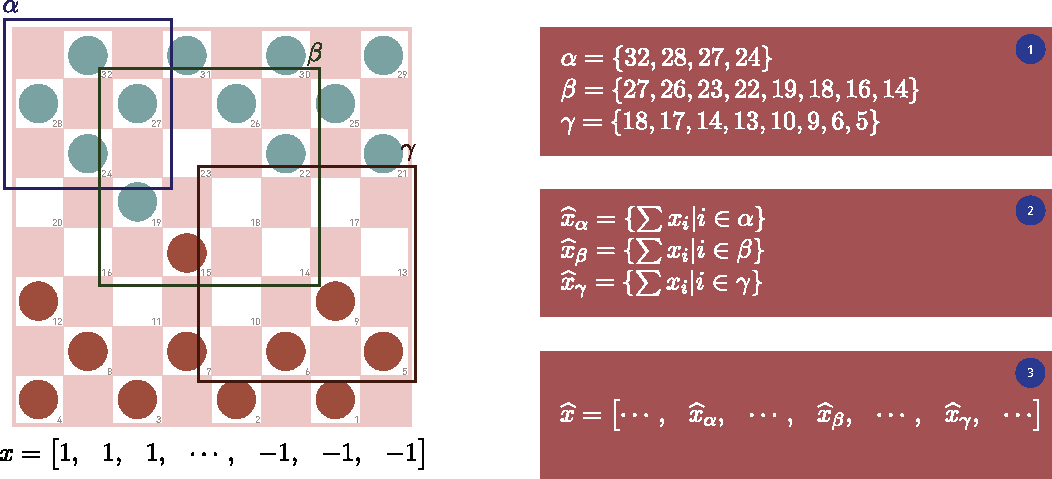
\includegraphics[width=130mm]{images/subsquares.pdf}
            \caption{A diagram visualising the processing of subsquares on board $x$ to create the preprocessed array $\widehat{x}$. Each index in $x$ represents a position on the board, such that each item in $x$ represents a value of the piece on the board. $\alpha$, $\beta$ and $\gamma$ are examples of 3x3 and 4x4 subsections. \label{subsquares}}
        \end{figure}

        % Talk about the activation function
        Weights $w$ of a neuron are multiplied by their input value $I$, summed with their bias $B$, and are passed through an activation function $O = f((I* w) + B)$ to become an input for another neuron. Activation functions, when visualised, usually have a sigmoid curve, but may also take the form of other shapes. Common characteristics of activation functions include values to be monotonically increasing, continuous, differentiable and bounded.
        % how does it work?

        % Tanh Diagram
        \begin{wrapfigure}{r}{0.4\textwidth}
            \centering
            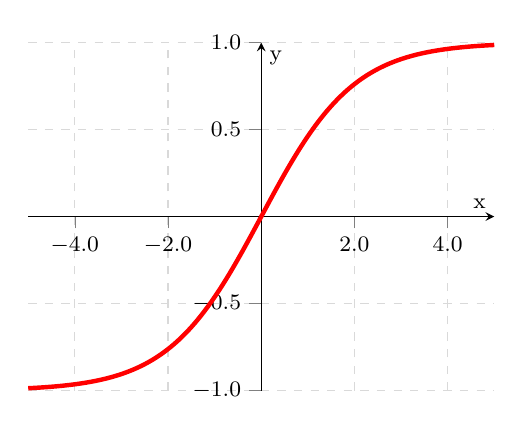
\begin{tikzpicture}
                \fontsize{8}{11}
                \begin{axis}[
                    legend pos=north west,
                    axis x line=middle,
                    axis y line=middle,
                    x tick label style={/pgf/number format/fixed,
                                        /pgf/number format/fixed zerofill,
                                        /pgf/number format/precision=1},
                    y tick label style={/pgf/number format/fixed,
                                        /pgf/number format/fixed zerofill,
                                        /pgf/number format/precision=1},
                    grid = major,
                    width=75mm,
                    height=6cm,
                    grid style={dashed, gray!30},
                    xmin=-5,     % start the diagram at this x-coordinate
                    xmax= 5,    % end   the diagram at this x-coordinate
                    ymin= -1,     % start the diagram at this y-coordinate
                    ymax= 1,   % end   the diagram at this y-coordinate
                    %axis background/.style={fill=white},
                    xlabel=x,
                    ylabel=y,
                    tick align=outside,
                    enlargelimits=false]
                % plot the stirling-formulae
                \addplot[domain=-5:5, red, ultra thick,samples=500] {2*(1/(1+e^-x))-1};
                % \addlegendentry{$f(x)=\frac{1}{1+e^{-5x}}$}
                \end{axis}
            \end{tikzpicture}
            \caption{Graph of tanh function $f(x)={\frac{2}{1+e^{-x}}- 1}$ (An example of an activation function with a sigmoid curve). \label{sigmoid}}
            \vspace{-10pt}
            \end{wrapfigure}

        Our choice for the activation function is tanh (a type of sigmoidal function), shown in figure \ref{sigmoid}. 
        % There exists inherent issues related to the properties of their derivatives, commonly known as the missing gradient problem. This is an issue  \cite{nair_rectified_2010}, described as the missing gradient problem. However, since this issue is related to the properties of a gradient based learning method and not through a stochastic learning method (of which genetic algorithms are), this is not a concern for the project. 
        The use of tanh facilitated the ability to simulate a zero sum formula (for a range of [-1 to 1]) due to its symmetric properties around the origin.
        
        Results are cached such that evaluations are saved such that they can be recalled immediately, in the event that the same input was evaluated again. This showed  varying levels of time improvement based on the ply depth. As the ply increased, the size of the state space increased, and therefore the chances of recalling the same set of inputs decreased. The cache was also used for our safe mutations algorithm, described later on in Section \ref{coefficient_mutation}.

        The neural network was implemented manually via NumPy to allow direct access to the weights, allowing the genetic algorithm access to manipulate them.
    
    % DONE
    \subsection{Decision Making Algorithm}
        Initially, the decision making algorithm implemented was the same mini-max approach as in Samuel's program \cite{samuel_studies_1959}, but was then progressed to a modified Monte-Carlo Tree Search (MCTS). A basic MCTS differs from mini-max where future moves are randomly played to the end of the game. It acts as a sampling of possible outcomes, and does not depend on an evaluation function at all. A survey found that MCTS can dramatically outperform mini-max based search engines in games where evaluation functions are otherwise difficult to obtain \cite{browne_survey_2012}. MCTS was played in rounds which consist of four operations:

        \begin{itemize}
            \item Selection: A selection strategy was played recursively until some position was reached. 
            \item Play-Out: A simulated game was played. Again, a basic form of MCTS would play until an end-game was reached.
            \item Expansion: A node was added to the tree.
            \item Back-propagation: The result of the game was back-propagated in the tree of moves.
        \end{itemize}

        These rounds are repeated until a certain period of time was met or a certain number of rounds are computed. Once finished, a node was chosen based on its total probability of reaching an winning outcome.

        \begin{figure}[!ht]
            \centering
            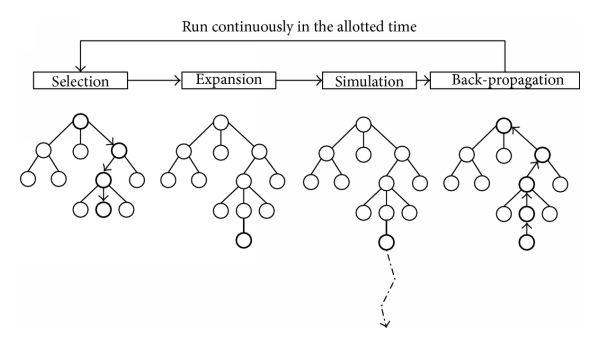
\includegraphics[width=100mm]{images/montecarlo.png}
            \caption{A diagram describing the MCTS process.}
        \end{figure}

        MCTS-EPT (or MCTS with early playout termination) modifies the MCTS random play-out approach. Instead of allowing the random moves play to the end of the game, the number of moves traversed are capped and an evaluation function (which was the neural network) was applied at that future state instead. \cite{lorentz_using_2016} The model was then adapted such that when the number of possible moves was less than 4, the ply depth would extend by the number of moves. This reduced the need to depend on random playouts of moves to the end state, and ensures that the quality of the moves was contingent on the evaluation function. For our results, we use the ply depths 1,3 and 6 to determine whether the system plays in a consistent fashion. As opposed to using a time threshold, the number of MCTS rounds $r$ was based on the ply depth $p$, such that $r=300p$. This allows the system to process moves in a manner that the performance of the system was hardware-independent, as faster machines could have processed more rounds within the same fixed set of time.

        % talk about the fact that this is a probabilistic strategy

        % The minimax algorithm would be retained to evaluate the performance differences between the two decision making algorithms.

    \subsection{Genetic Algorithms}
        % talk about generation of population
        % talk about tournmanent
        % talk about 
        The genetic algorithm (GA) was the premise of the system's learning strategy. GAs are used to train the neural network. We discuss the various algorithms that form the collection of GA strategies below. For the system, a population size of 15 was chosen, due to the restraints on available computational performance.

        \subsubsection{Population Generation} \label{population_generation}
            % Introduce what its for
            In genetic algorithms, the population serves as a base that allows agents in the pool to play each other. Every generation has its own population of agents, and the population size was consistent across the generations. The initial population consisted of randomly generated weights and biases of the neural network, with values from [-1,1]. 
            
            For a population size of 15, the next generation was created using the best five agents from the current generation (discussed in {\it{\ref{tournament_selection} Tournament Selection}}.) They would continue to play in the next generation; this strategy is described as elitism. The next eight players were generated through the use of crossover strategies (see {\it{\ref{crossover_strategy} Crossover Strategy}}). The weights of the $1^{st}$ and $2^{nd}$ place agents are used as inputs to the crossover strategy and generated 4 off-springs. Two were reciprocal crossover representations of each other, and the other two being directly mutated from the parents themselves. Another four children are created using the same strategy, with the 2nd and 3rd agent's weights. The remaining two were direct mutations of the 4th and 5th place agents.

        \subsubsection{Tournament Selection} \label{tournament_selection}

            To sort the quality of the players in a population, a tournament selection process was deduced. This allows us to choose the best players who will continue to play in the next generation.

            Each agent in the population plays a minimum of 5 games as Black, against randomly selected opponents. Each game lasts a maximum of 100 moves from both players. If a winner was not deduced at this stage, a draw was called. Draws are also called when there was a three-fold move repetition from both players. A win was worth $2$ points, a draw being none and a loss being $-1$ point. Both the agent and its opponent receives a score from the game.
            Scores were then tallied up at the end of the tournament. Players were sorted by the number of points they scored. The best players had the highest number of points.
  
            All of the games were run in an 'embarrassingly parallel' fashion through the use of Python's multiprocessing library. Whilst the league structure was found as the better approach \cite{al-khateeb_introducing_2009} it would increase the overall running time as the initialisation of some games are dependent on the outcomes of other games. This lead to a longer overall running time even though less games are played, whereas the embarrassingly parallel method allowed every game to play simultaneously.
            
        \subsubsection{Coefficient Mutation} \label{coefficient_mutation}

            \begin{figure}
            \begin{equation}
                % \caption{The mutation formula. \label{mutation}}
                w_n = w_p + \frac{m}{\sqrt{2 * \sqrt{K} }}
            \end{equation}
            \caption{The mutation formula, where $w_p$ is the current weight, $K$ represents the number of weights and biases in the neural network, and $m$ representing a random floating point in the range of [-1,1].\label{mutation}}
            \end{figure}

            To create variation between agents and their offspring, statistical anomalies are made through the use of mutations. This was used as one of the learning mechanisms that help change the decision factors of the neural network. Weight and biases of an agent's neural network would increment by a random value that was created using the equation in Figure \ref{mutation}.

            Like the activation function,
            % (in \ref{sigmoid})
            the weights would have a soft maximum of [-1, 1]. This consequently meant that the mutation was not controlled, but rather dependent on the number of weights in the system; The more weights in the network implies a less significant mutation. Soft mutation \cite{lehman_safe_2017} was also used. We use a subset of historical neural network calculations as a premise to guide our mutation. The method is as follows:
             
             \begin{enumerate}
             \item With the current set of weights $w$, choose a subset of pre-calculated input and output tuples $\phi_{w} = (I, \lambda_{I,w})$ where $I$ represents the input values of the network, and $\lambda_{I,w}$ as the output.
             \item Generate a perturbation $y$ of the weights calculated using the formula in Figure \ref{mutation}. Use $y$ as a basis of a neural network. 
              \item Using the inputs $I$ in $\phi_{w}$, calculate a new set of input and output tuples $\phi_{y} = (I, \lambda_{I,y})$.
              \item Calculate the divergence $\delta = \lambda_{I,y} /\ \lambda_{I,w}.$ 
              \item Calculate the quality of $y$ based on the number of inequalities $\delta \geq 1$.
             \item Repeat parts 2-5 some $n$ times, keeping note of the the best $y$. 
             \end{enumerate}

            The intuition behind this was that if $\phi_{w}$ was a subset of moves that led to a winning game, then the manipulation of the weights was left open as long as it can replicate the performance of winning games.
            
        \subsubsection{Crossover Strategy} \label{crossover_strategy}
      
           \begin{figure}[!ht]
                \centering
                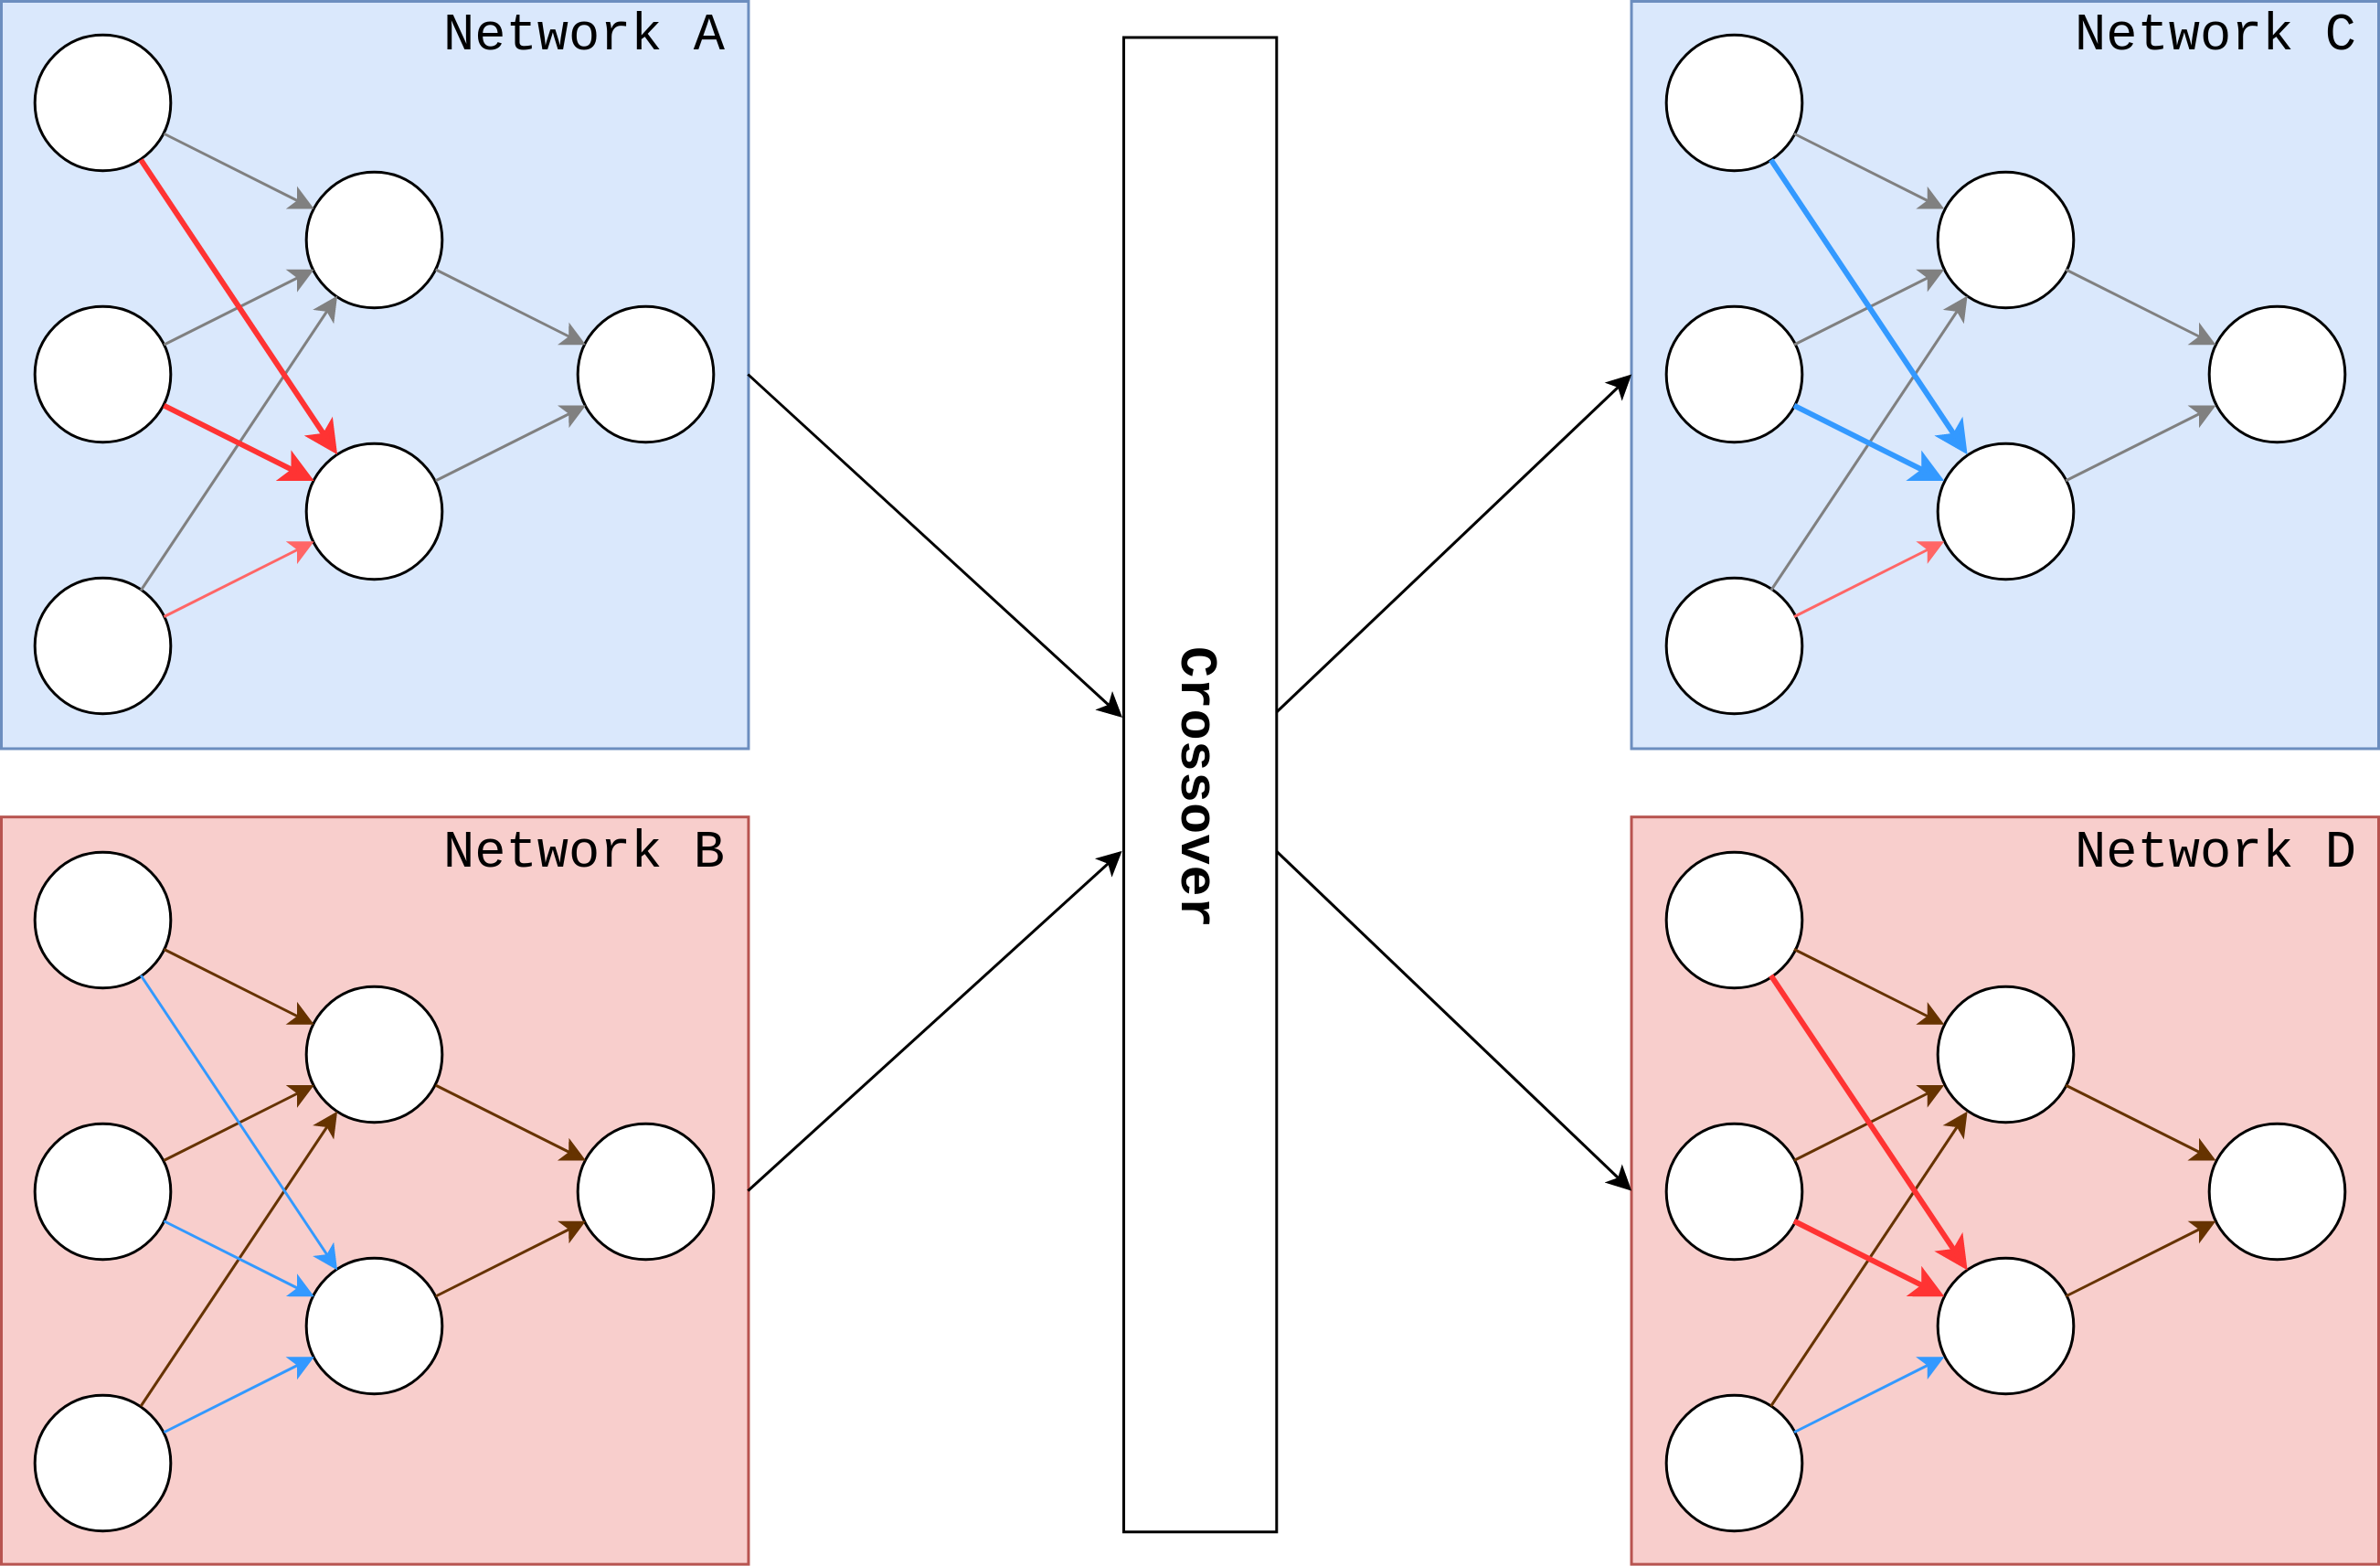
\includegraphics[width=80mm]{images/crossover.png}
                \caption{A diagram visualising the crossover process.\label{crossoverpic}}
            \end{figure}

            The distinct learning mechanism unique to genetic algorithms was the use of crossovers. This combines the traits that build two parent agents to create children. In our scenario we use the weights and biases of the parent's neural networks.

            Two off-springs were created from a pair of parents, with each offspring being the reciprocal crossover of each other. 
            % The weights of both parents (now each treated as a 1D array of coefficients), are divided contingent on the number of weights and biases for a given layer. Each layer should be treated separately to reduce the potential dependency on a purely randomly generated neural network. For each set of weights in a given layer, Algorithm \ref{crossover} describes the crossover process in pseudocode.
            A random node from the dominant parent was chosen. A dominant parent was the agent who gained more points in the tournament round than the other (who would be the submissive parent). If a dominant parent cannot be deduced, it would be randomly chosen. 

            Once a node was chosen, a subset of weights and biases that are fed into the chosen node are swapped with the submissive parents values at the same positions. As values in the weights can range from -1 to 1, dominant input weights are values that are greater than 0.75 or less than -0.75. Figure \ref{crossoverpic} visualises the process. In the diagram, Network A and B are parents, creating reciprocal offspring networks C and D. A was the dominant network, and A's node with the red inputs was chosen. The weights and biases of the red inputs are swapped with the values at the same position in network B. Network C was formed with Network B's dominant weights, with the rest being composed from A. Network D was the reciprocal, having Network A's dominant weights and the rest from B.

            The crossover should create a subtle modification to a neural network, by swapping a small subset of weights and biases at a time. Having a more dramatic crossover could potentially change the structure of the network flow, reducing its effectiveness. 
            
            % Talk about how this is not commonly used.

    \subsection{Testing}

        At the end of a given generation, we measure growth of performance by using the generation's champion. When a new champion was generated, it was played against the previous 5 champions from earlier generations. 6 games are played for each previous champion, with 3 being as Black, and 3 being White. A mean score was calculated from those 6 games. The overall performance of the current champion was the mean of the 5 sets of games. A positive improvement was when the mean of means are greater than 0. Point Score for the champion games are measured by {1,0,-1} where a Win counts as 1 point, 0 for a draw, and -1 for a loss. The weights are scaled differently to the regular tournament in order to portray an even distribution of the learning rate.
    
        \subsubsection*{Evaluation Method}
    
        The end player, representing the champion at the last generation, was used to create comparison games against its ancestors. This player was to be first tested against an agent who was choosing random moves to verify that the system was not playing in some random fashion. Measurements from these games, alongside its champion scores be used as evidence to determine whether the agent was learning over time, was used to answer to answer the research question.
       
    \subsection{Tools}
    % Description of tools used
        The system was built using Python 3.6 and the \inlinecode{Python}{NumPy} library. Initial runs operated on a 1 and 2-ply load to determine the stability of the system. As the memory usage of the system was negligible, it was not considered when choosing hardware. This was run on a linux (Ubuntu) machine containing a 4-core Intel i5 6600u processor. Development and debugging was also handled on this machine. Once testing has shown to be stable, the system was then configured to run on Durham's MIRA distributed system (Debian). MIRA contains 4 Intel Xeon E7-8860 CPUs (Each CPU contains 16 physical cores running in 2.2Ghz, with hyper-threading). This comes to a total of 64 Cores, and 128 threads. The \inlinecode{Python}{multiprocessing} library was used to run the tournaments in parallel. To interpret the results, charts are generated at the end of every generation using \inlinecode{Python}{pyplotlib}.
        
        A consistent SSH connection was used to ensure the simulations were kept alive for the duration of the simulation on MIRA. Once training was complete, performance measurements was also conducted on MIRA, alongside other statistical evaluations to reduce computational time. The end champion was then transferred to the initial testing machine to be played against human input.

    \subsection{Verification and Validation}

        Each component of the system, such as the neural network, MCTS, and genetic algorithms, were built in their own classes. This helped to achieve two things; unit testing, and modularisation. The use of unit testing (performed per class) helped to verify that individual components worked as expected, especially with a project of this scale. Components that are shown to work are then added to the system. Training the system takes a while (discussed further in Figure \ref{cpu_table}, and realising errors was a notably laborious task. Modularisation of the code allowed for quick deployment of new features, such as migrating decision making algorithms.

        %  Reducing the time involved in debugging allowed for more time for training.

    % Issues
    \subsection{Issues}
    %   discussion and testing
        Verifying that the moves are properly chosen was difficult and slow, as games need to be played out first, with the quality assurance handled afterwards. The main issue with implementing the system were two-fold. The main issue was the sensitivity of the program, which was compounded by the time spent in terms of realising issues with the implementation. There are no obvious clues to analysing why the system may not perform as expected due to the scale of the system, and the issues are not realised until some time was spent during simulations. 

        Although the system was built where the games in the tournaments are "embarrassingly parallel", the machine used for training did not scale as efficiently as expected. Most of the computation was spent on calculating floating point matrix operations (Which represents the neural network evaluations.) Later research has shown that the use of hyper-threading does not necessarily show to scale the performance, even though more threads exist. \cite{leng_empirical_2002} This was due to the shared floating point arithmetic registers in the CPU, where two threads utilise the registers of one physical core. The use of GPU acceleration was not considered due to the lack of availability, and the added complexity involved for its implementation. 
    
% TODO (WAIT FOR RESULTS)
\section{Results}
    %   Results:
    %   - Does it work?
    %   - Perhaps some measurable outcomes where appropriate.
    % this section presents the results of the solutions.  It should include information on experimental settings.  The results should demonstrate the claimed benefits/disadvantages of the proposed solutions.
    

    % This section should be between 2 to 3 pages in length.
    % need to talk about how we mwasure the success of the system
    For the experiment, we create three different neuroevolutionary systems, each having different ply-depths: 1,3 and 6. All systems run for 200 generations. For Figures containing three charts, each chart represents the results of the agents playing at 1-ply, 3-ply, and 6-ply, respectively. Each simulation utilises a population of 15 agents.

    \subsection{Learning Rate}
    % chart of performance over time
    
    The learning rate was derived by comparing the i$^{th}$ generation's champions with its predecessor champions from the previous five generations [$i-1, \cdots, i-5$]. For each previous champion, six games are played, with the outcome of the current champion's performance scored and tallied up. An average of the outcomes was deduced, representing the learning rate. The learning rate of the first 2 champions were not measured due to insufficient comparisons. This measurement was performed for every generation until the end of training. These measurements do not influence the actual learning process of the system, but was used as one of the indicators of whether the system was learning in ability over time, i.e. whether the new champion was better than its predecessors. These results are plotted cumulatively to show the overall learning rate.
    
    \begin{figure}[!ht]
        \centering
        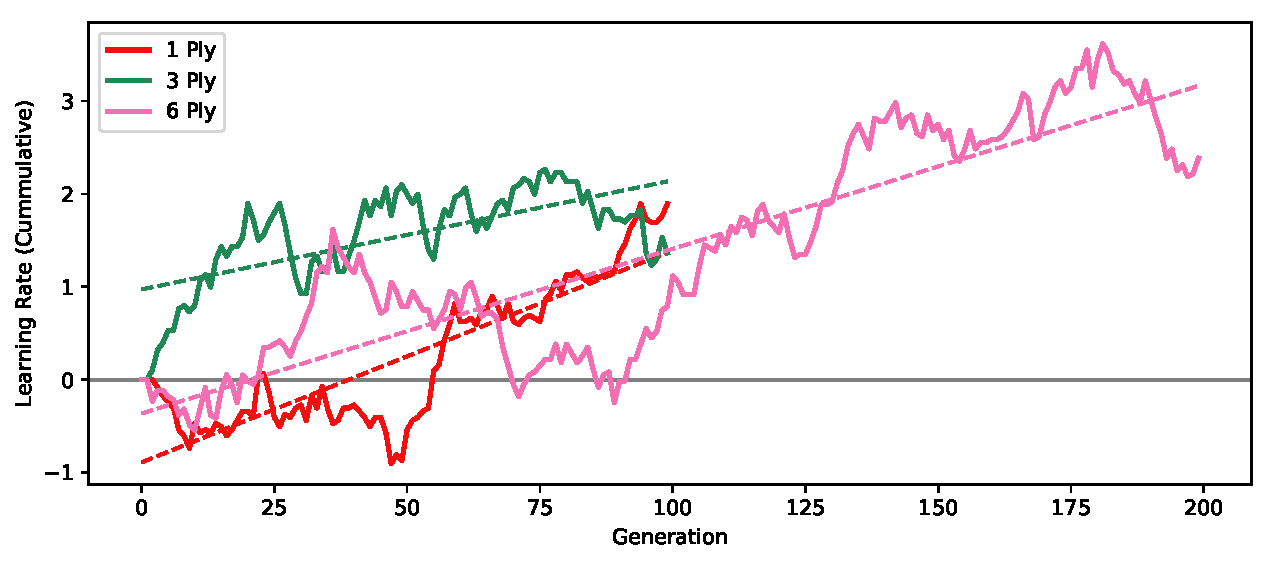
\includegraphics[width=160mm]{images/results/combined_cummulative.pdf}
        \caption{A chart showing the cumulative learning rate across the generations for the different ply depths.\label{cum_growth}}
    \end{figure}
    
    A cumulative growth across all ply depths can be seen such that returns are in the net positive as more generations are added. Interestingly, the 3-ply shows a slower learning rate than the other plys. However, even with safe mutations, we can also see that the performance over time was very volatile for all plys. This could potentially be prevented by creating a new set of agents and restarting the generation's tournament when a loss was seen. Further measurements are taken to understand the reasoning of the potential troughs in performance. 
    
    \subsection{Performance}
    To measure the overall system performance, the champion of the final generation was compared against a subset of their much earlier predecessors to measure the retention of move heuristics over time. For each predecessor, the trained system played 128 games (half as black and the other for white), and the number of wins, losses and draws were counted. For debugging purposes, all agents played against a randomly playing program to determine whether the system correctly evaluated moves. A trend line was produced (with a cubic best fit equation) for the non random games.
    % compare the bots against a minimax agent
    % chart of previous champions
    \begin{figure}[!ht]
        \centering
        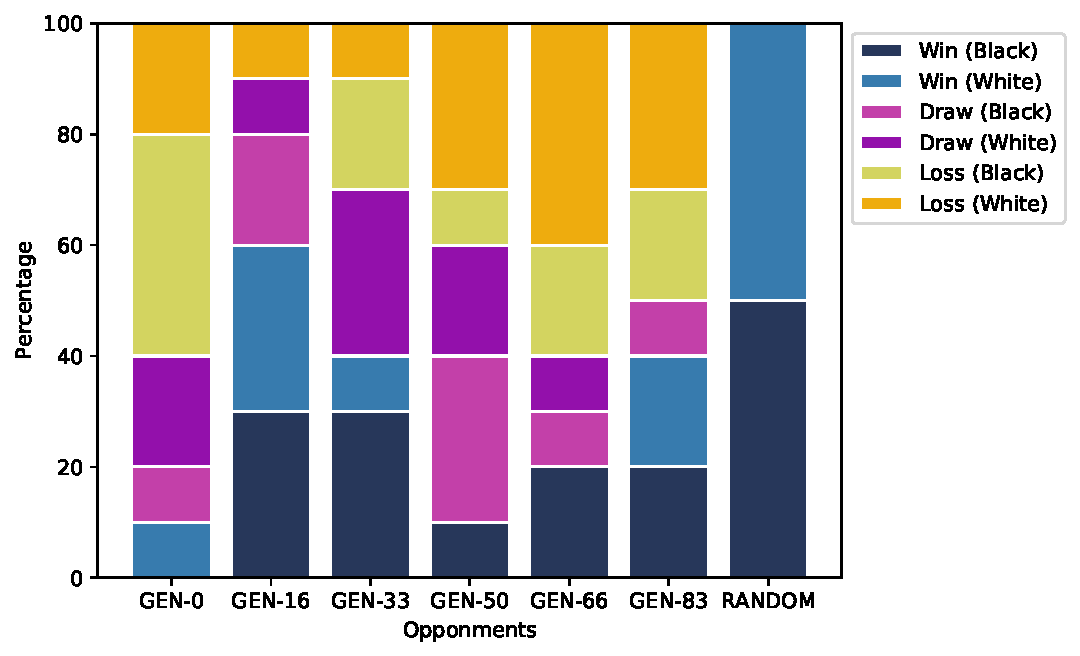
\includegraphics[width=53mm]{images/results/1ply/gm_net_stats.pdf}
        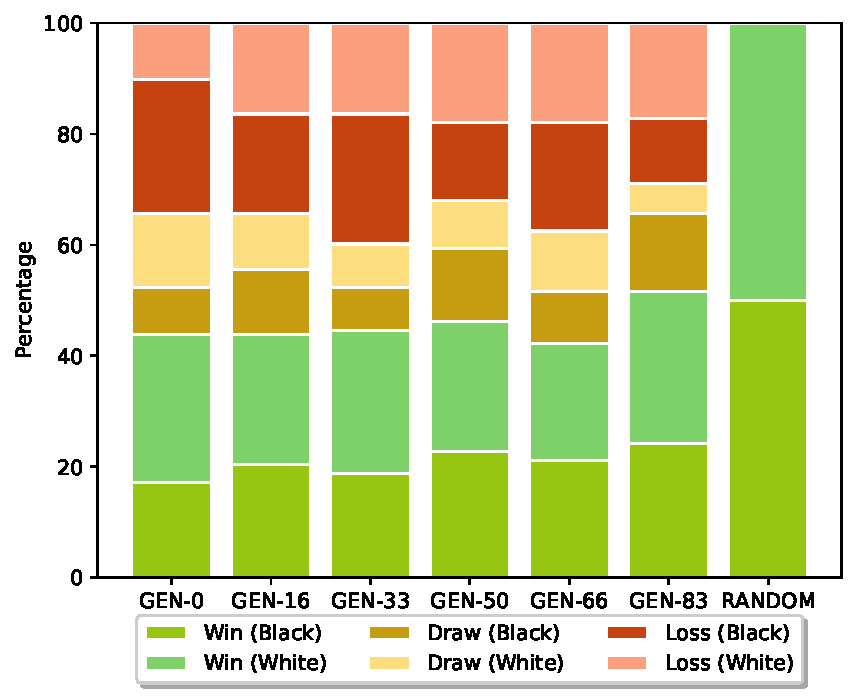
\includegraphics[width=53mm]{images/results/3ply/gm_net_stats.pdf}
        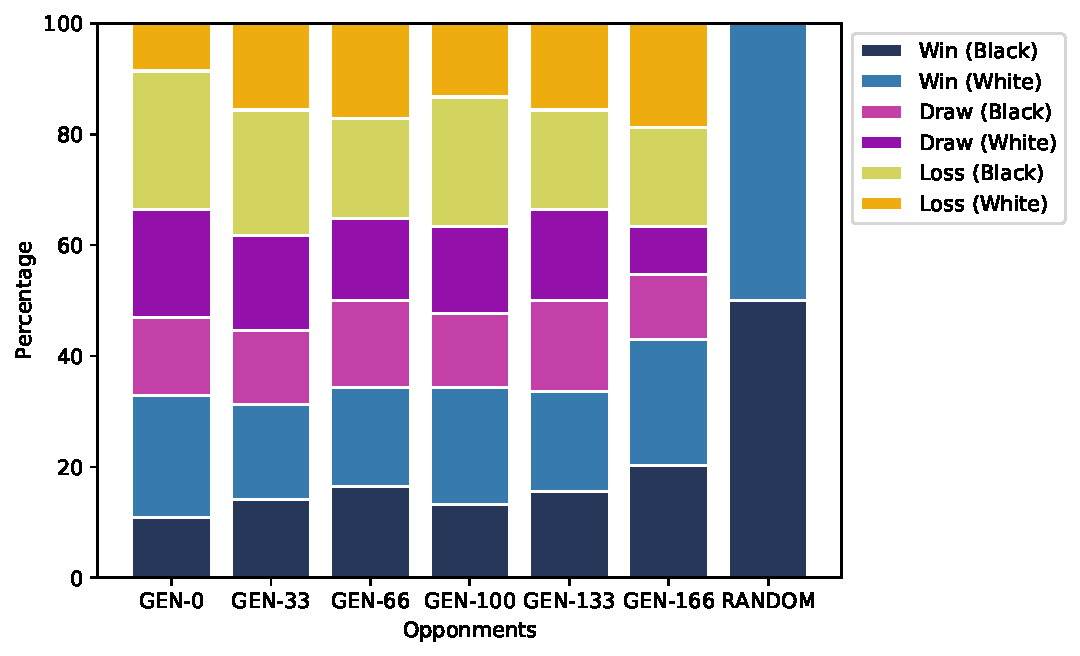
\includegraphics[width=53mm]{images/results/6ply/gm_net_stats.pdf}
        \caption{Charts showing the performance of the trained systems against their ancestral counterparts.\label{net_stats}}
    \end{figure}
    
    For all systems, it appears that the winning rate increased over time, with the draw rate and loss decreased over time. For ply depths 3 and 6, it performed significantly better than it's generation 0 counterpart (when considering the percentage of losses). This was not the case for the 1-ply - where it lost more frequently than its wins and draws combined - against its generation 0 counterpart. This would be caused by the lack of oversight heuristics retained as the system does not look ahead further enough to decide what heuristics would be kept by the neural network model.
    % For the ply depth of 1, we can see an immediate net trend, with the end system beating earlier generations except for the first generation. 
    % % bollocks
    % This makes sense, as heuristic retention would be lost as the search depth is so low. This does however suggest that the system is worse off than playing with an initialised system (without training). For the higher ply depths (3,6) however, the agents managed to consistently maintain a higher chance of winning/drawing against their earlier counterparts. It is difficult to see a trend line that suggests the growing performance of the systems over time. 
    % A decreasing trend line for draws 
    % Need to talk about losses for the 6-ply

    \subsection{Champion Distribution}
        Measurements are taken to show the genome type distribution of the champions across the generations.
        This was to determine whether the champions were more likely to be chosen based on the influence of mutations and crossovers. Each of the champions were looked at, and their genomic properties were collated to show a distribution of the chances of a particular agent being the champion. Champions that were also champions from prior generations are classed as persistent. Well performing agents from previous generations (but not champions) are classed as elitism. Typically, elitism would encompass the persistent agents but for the sake of measurements they were taken separately. This was also the case for mutations; Although every offspring was mutated, some of the offspring were created using genomic crossovers (which were also classed separately), described in section \ref{crossover_strategy}.  

        \begin{figure}[!ht]
            \centering
            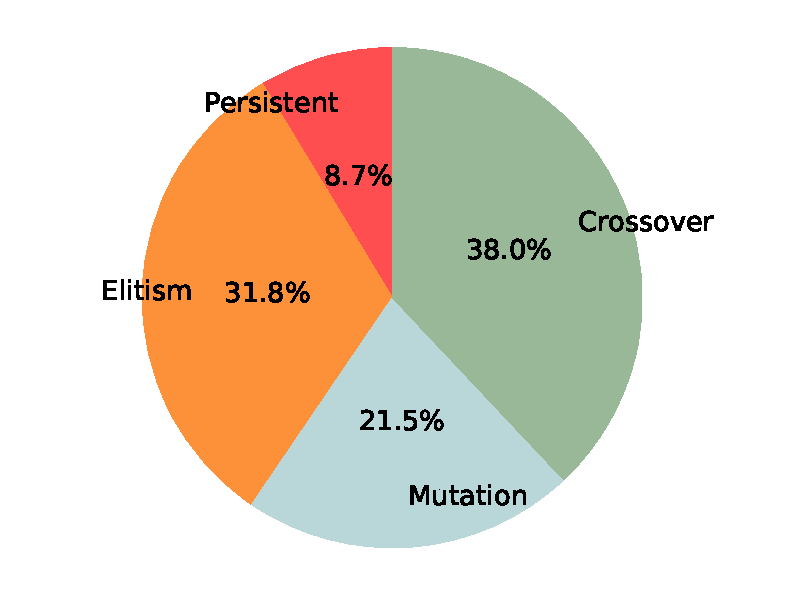
\includegraphics[width=53mm]{images/results/1ply/champ_gen_dist.pdf}
            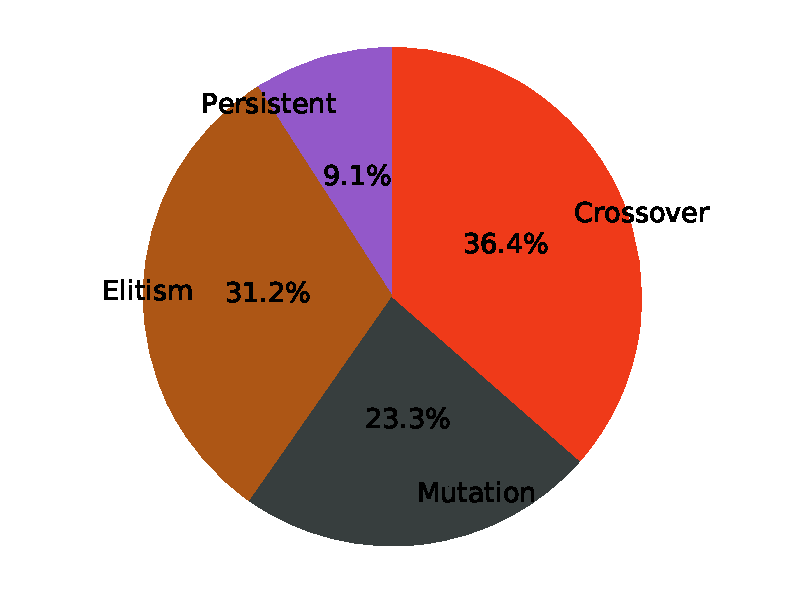
\includegraphics[width=53mm]{images/results/3ply/champ_gen_dist.pdf}
            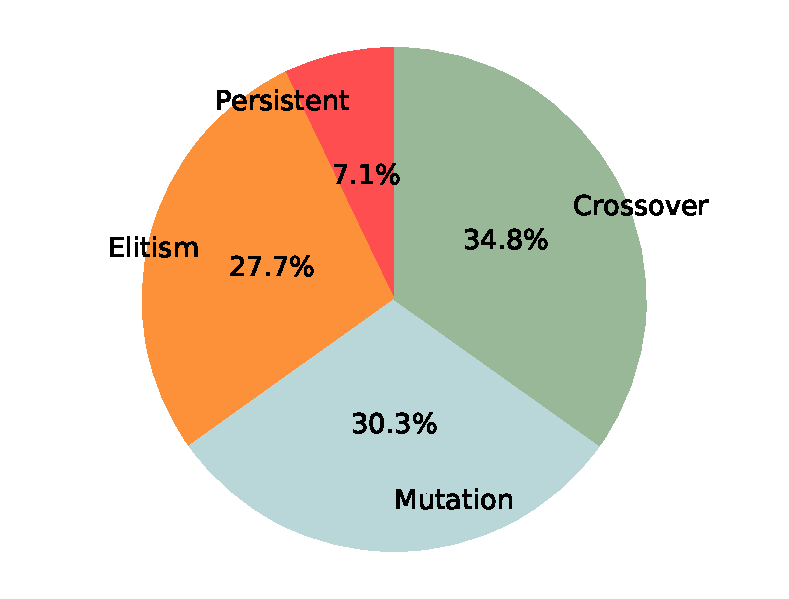
\includegraphics[width=53mm]{images/results/6ply/champ_gen_dist.pdf}
            \caption{Distributions of the different genomic identities across the tournament champions. \label{champ_gen_dist}}
        \end{figure}

        Interestingly, the influence of crossovers reduced when the ply depth increased, and the influence of mutations increased across the generations. Overall however, crossover holds the highest probability across the ply depths which would suggest that the use of crossover methods (the distinctive feature of genetic algorithms opposed to other evolutionary methods) combined with mutation, would increase the chances of producing champions. The influence of the learning components of genetic algorithms (crossover and mutation) increased in relation to the increasing ply. (representing 59.5\%, 59.7\% and 65.1\% of the distributions, respectively.)

    \subsection{Quality of Inheritance Methods}
        Building on from the chart provided by Figure \ref{champ_gen_dist}, we look into the scores retrieved by the different genomic identities when they are compared against their earlier counterparts. This determines whether the use of genetic algorithms can overall improve the quality of neural networks. To measure this, we correlate the generation's champion with their score (the same measurement used to evaluate the learning rate in Figure \ref{cum_growth} produced when measured against their predecessors. The results are shown in Figure \ref{champ_score_distribution}. Red circles indicate individual values for their classes.

        \begin{figure}[!ht]
            \centering
            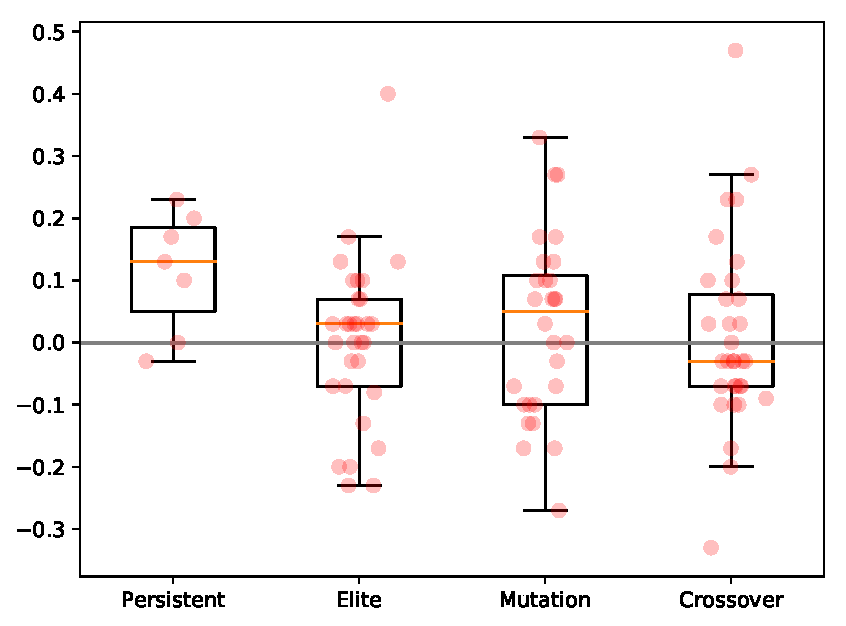
\includegraphics[width=53mm]{images/results/1ply/champ_score_distribution.pdf}
            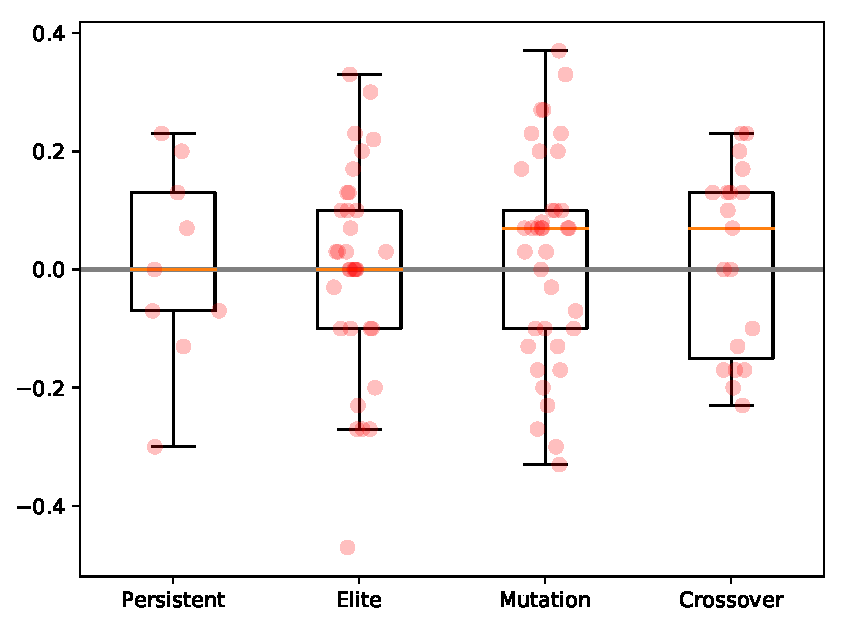
\includegraphics[width=53mm]{images/results/3ply/champ_score_distribution.pdf}
            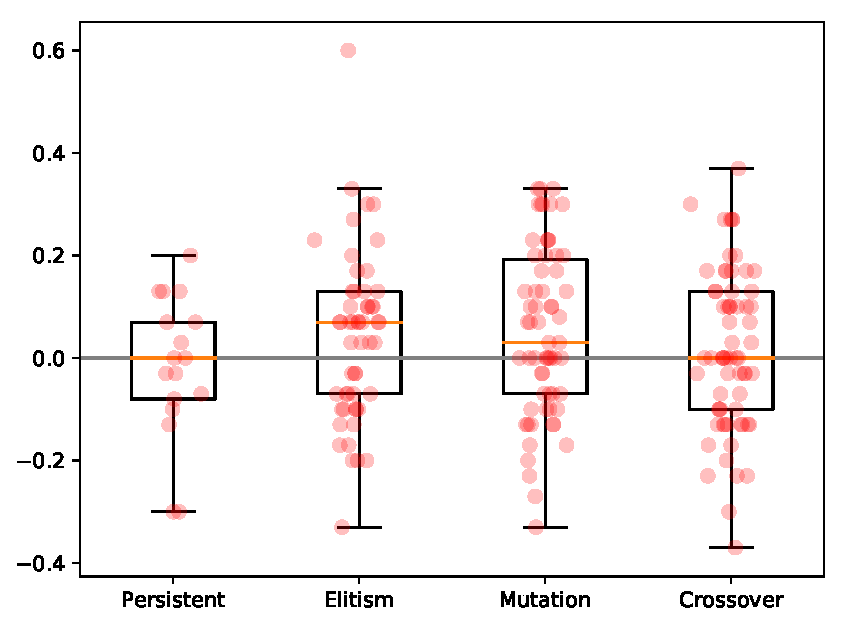
\includegraphics[width=53mm]{images/results/6ply/champ_score_distribution.pdf}
            \caption{Box-Plots of the different genomic identities and their distribution of scores. The yellow line in the box represents the mean score. \label{champ_score_distribution}}
        \end{figure}

        Unsurprisingly, crossovers had a larger range of possible values compared to its mutation counterparts. This was most likely due to the weights being placed at different positions on the neural network, disrupting any heuristics it would have otherwise devised. However, the mean crossover score suggested that it negatively impacted the learning rate. Furthermore, the range and mean scores for the elitism genomes (Persistent agents and elitism) suggests that they were more likely to increase the learning rate.

    \subsection{Other Observations}
        \subsubsection{Number of Moves}
            The number of moves was measured to verify the system was able to produce quality moves across the training phase. Figure \ref{move_chart} show the distribution of moves for the games played over the generations.

            \begin{figure}[!ht]
                \centering
                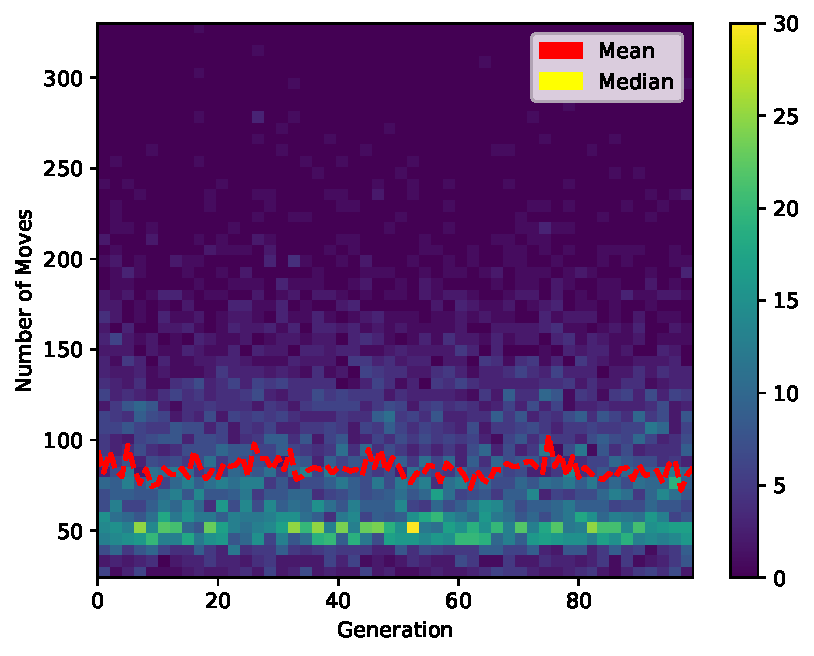
\includegraphics[width=53mm]{images/results/1ply/moves.pdf}
                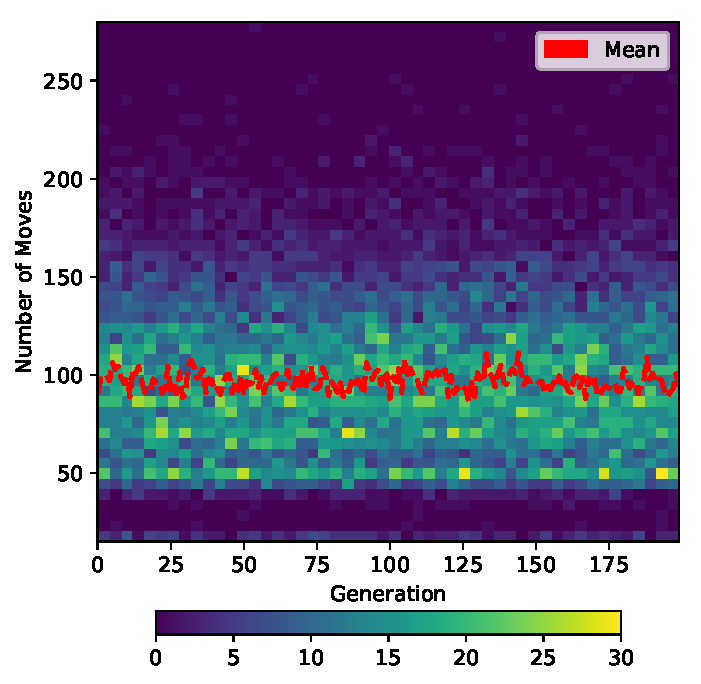
\includegraphics[width=53mm]{images/results/3ply/moves.pdf}
                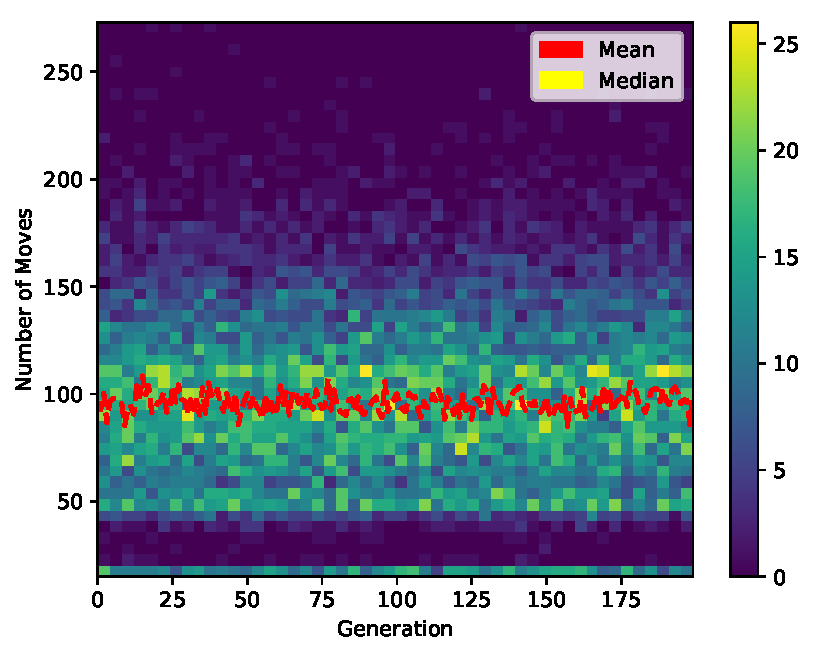
\includegraphics[width=53mm]{images/results/6ply/moves.pdf}
                \caption{2D Histograms representing the number of moves played in the games played in the generations. \label{move_chart}}
            \end{figure}

            % The number of moves is consistent throughout as the players are evaluating by projecting their own abilities to the opponment, leading to a fairly even distribution of moves across the generations. 
            From the charts, the median number of moves in a game for 1-ply was around 50. 
            For the higher plys, the median was not as tightly grouped together. When combined with the mean number of moves, suggests that when both players were creating stronger quality decisions when playing the game, the games lasted longer. The mean number of games for both 3 and 6 plys are very similar. However, the similarity of the two charts was most likely caused by the hard limit imposed by the game rules, where draws were forced when a piece was not taken after 100 moves. 
            As the system was shown to scale in quality of moves across the generations, this verified that the system was choosing moves at a consistent quality throughout. This consequently confirmed that the decision making algorithm was implemented correctly, reducing the unknowns considered during evaluation.

        \subsubsection{CPU Times}

        \begin{figure}[!ht]
            \centering
    
                \begin{tabular}{ccccc}
                       & 1-Ply        & 3-Ply          & 6-Ply          & \\ \cline{2-4}
                \multicolumn{1}{c|}{Mean} & \multicolumn{1}{r|}{0:04:24} & \multicolumn{1}{r|}{0:17:32}  & \multicolumn{1}{r|}{0:38:45}   & \\ \cline{2-4}
                \multicolumn{1}{c|}{Net} & \multicolumn{1}{r|}{7:21:25} & \multicolumn{1}{r|}{1 day, 5:14:41} & \multicolumn{1}{r|}{5 days, 9:12:25} & \\ \cline{2-4}
                       &          &           &            & 
                \end{tabular}
    
            \caption{Mean and Net running times of system training for the various depths. \label{cpu_table}}
            \end{figure}


            To measure the time complexity of the program, time measurements were taken for every game played, and the time length for a generation to finish the tournament. As expected, 
            % rewrite it doesn't even make sense
            the system was shown to scale in a relatively linear fashion according to Figure \ref{cpu_table}. This was most likely caused by growing the search limit for MCTS in a linear fashion based on the ply-depth.

            \begin{figure}[!ht]
                \centering
                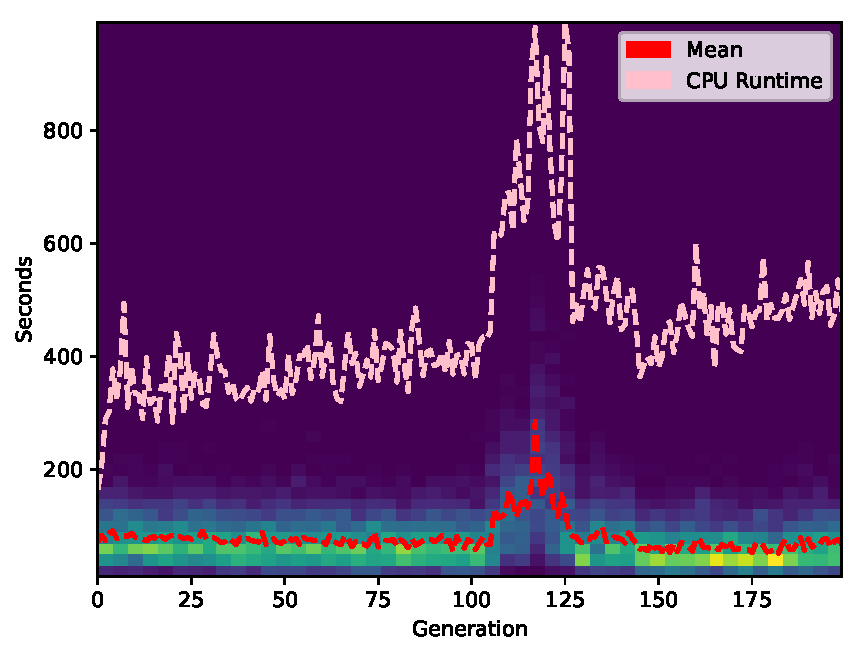
\includegraphics[width=53mm]{images/results/1ply/simulation_timings.pdf}
                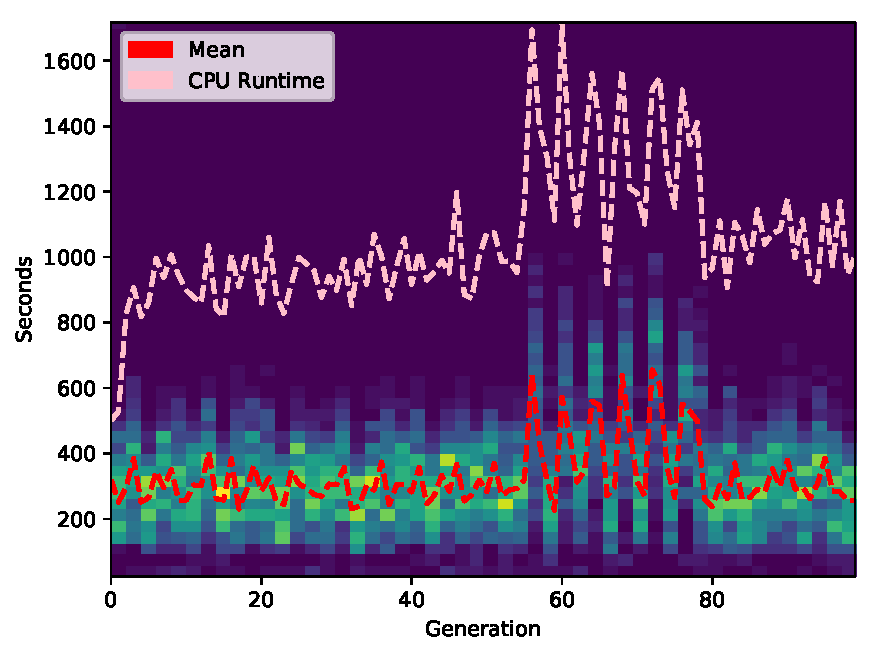
\includegraphics[width=53mm]{images/results/3ply/simulation_timings.pdf}
                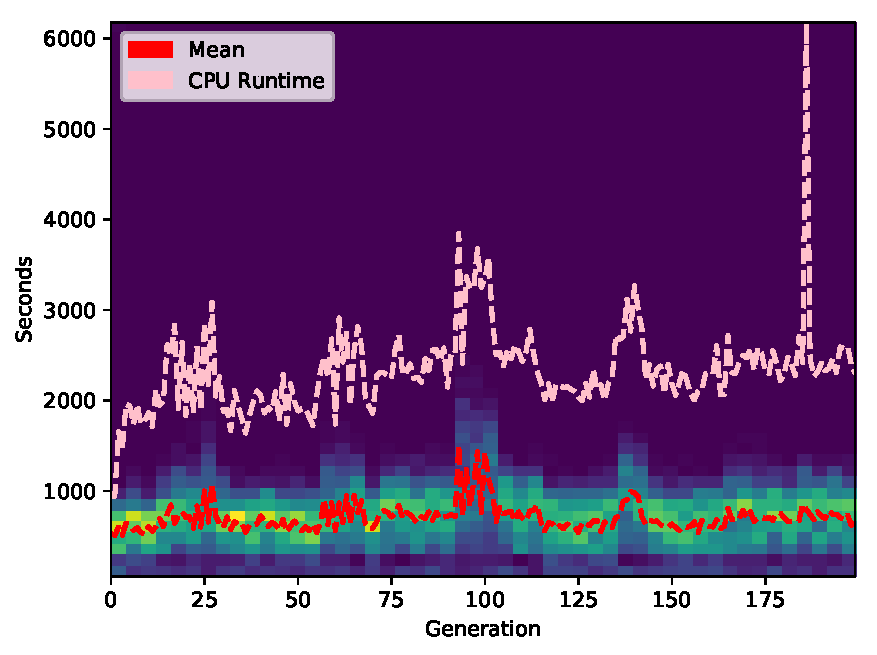
\includegraphics[width=53mm]{images/results/6ply/simulation_timings.pdf}
                \caption{2D Histograms of the average times spent on the games during the simulations. \label{chart_cpu_times}}
            \end{figure}

            Figure \ref{chart_cpu_times} suggests that the CPU time was very unstable during training, but further analysis suggested that it did not correlate with the performance of the system. This was most likely related to the use of a time-shared machine (Durham's MIRA) to run the simulations, which may throttle the amount of resources for the system for other users with their own programs. %so what?

% TODO (WAIT FOR RESULTS)
\section{Evaluation}
    % Structure and content very project-dependent.
    % Follow the Design Report. Use the feedback.
    % Rule of thumb:
 
    %   Evaluation:
    %   - How well does it work?
    %   - Does it do what you wanted it to do?
    %   - How well did you do?
    %   - Did the plans pan out?

    We now reflect back to the original research question: "is it possible to create a performing draughts playing agent by the use of Genetic Algorithms and Neural Networks?".  We answer this through examining of the strengths and limitations of the system. 

    \subsection{Strengths}
    Because the agents are essentially playing itself to learn over time, no training data is necessary for the program to evolve itself. This relates to the fact that an infinite number of games can be simulated. The use of crossovers, which differentiates genetic algorithms and its other evolutionary algorithms has shown to improve the quality of the players, especially the case in the 3-ply.
    
    This suggests that neuroevolution is a viable method for problems with vast search spaces, or problems where data is hard to access. Although this is the case for Deep learning and evolutionary computation in general, the benefit of using genetic algorithms is that the system relies on a relatively simple learning heuristic that is open to domain specific adaptation. Gradient based learning requires the function  translatable to some form of a differential sum of partial derivatives, which may not be feasible in some circumstances.

    \subsection{Limitations}
    The results show a slow learning rate than typical ventures as there is an immediate comparison to make against, and requires many more samples (often exponentially more) to get a weight of equivalent quality.
    The quality of the neuroevolutionary algorithm boils down to the quality of the fitness function, which in our case is the tournament method. Round-Robin is not necessarily the most efficient (from a number of games played perspective, and not necessarily parallelism) and does not eliminate cases where there is an ambiguous decision between the champions (which could be due to several players having an equal number of points). One of the issues of the approaches taken in the paper is that when compared to agents from much earlier predecessors, some of the characteristics of the neural network used to win against them are lost. This was especially the case for the 1-ply program, where it performs worse than an randomly initialised agent. Creating a high quality fitness function is difficult and its domain specific, or rather, there is no universal fitness function for all problems. This poses as a benefit and a weakness for the neuroevolutionary approach.
   
    The crossover mechanism is a hit and miss, and is shown to impede the learning rate for some of the longer ply-depths. This may be due to its disruptive nature, as heuristics are destroyed. As feared by findings by \cite{emmanouilidis_comparison_2000}, we can see the potential fears of the negative influence of the textbook crossover mechanism, where it has shown in the results to discourage learning.

    % could not run for a larger population
    % restricted to not strong computers
    % lots of tweakable compomnents with not enough time to work on which could otherwise improve the performance
    % did not experiment with other dicision making algos which could further speed up performance
    % crossover had a wide range of values, and was on average shown to show no difference or negative difference, even though it was most likely able to become champions.

    % ---------------------
    % The challenge with all GA work is finding the right fitness function. If you don't understand your domain well enough to define a good fitness function you're going to be wasting your time, and no amount of algorithmic and/or AI magic is going to help you.
    \subsection{Approach}
        The modularity of the system implementation was pivotal to debugging the system. The program itself is quite sizeable, and it helps that individual tests can be conducted in most cases. It also helps that the order of the implementation helps.

        Measuring the learning rate is quite difficult and arbitrary, and may best be compared to against systems that are classified to play at a particular level. 

        As most of the experiments are constrained by computational power and time, it may be best to re-evaluate this concept until either computational resources are more available, such as the use of GPU acceleration. The system should also be left to run for longer generations as presently the results do not show a notably strong correlation. The lack of computational resources also influenced the number of experimental testing that can be measured, such as the population size, the number of generations and the learning rate. 
        
        Another consideration for the project is to experiment with different crossover algorithms that utilise the temporal difference between inputs and outputs. This could assist in the creation of safe crossovers which could also potentially accelerate the learning rate, by retaining the best aspects of two agents.
        
        There is an incredibly vast scope of future work that would extend the project. One interesting avenue is to consider using a safer method to produce mutation, exercising other contemporary methods in machine learning. It may also be the case that more time could be spent in examining references outside of computer science. In this particular example, the algorithms used are inspired by various biological and neuro-scientific understandings. More research into this field may assist in finding more creative methods of solving some of the issues concerning genetic crossover mechanisms and mutation rates.

% TODO (WAIT FOR RESULTS)

\section{Conclusion}
    % This section summarises the main points of this paper.  Do not replicate the abstract as the conclusion.  A conclusion might elaborate on the importance of the work or suggest applications and extensions.  This section should be no more than 1 page in length.

    In terms of fulfilling its objectives, the project was an overall success. A system was implemented using evolutionary methods and it successfully plays checkers in a manner in which it can learn from over time. To the extent of its growth remains suspect however. Efforts to measure the learning rate is one of the non-trivial challenges that makes neuroevolution a particular field of interest, as it is inherent that it can tackle problems in a somewhat novel manner.
    
    The main findings of this project is as follows:
    \begin{enumerate}
    \item It is evidently possible to create a checkers playing agent that learns to play itself, with little human intervention.
    % - some of the the work is 
    \item  neuroevolution is inefficient compared to their gradient based counterparts. This however was understandable due to the heavy dependency of entropy disguised as learning.
    \item  The fitness function can be anything, but it is important to derive a high quality fitness function.
    \item The quality of crossovers can be a deciding factor in how the agents learn to play over time.
    \end{enumerate}

    The major implication is that it is a possible contender for tasks that require unsupervised learning, and that the fitness function cannot be trivially decomposed into set of derivatives that allow regular derivative based learning to shine.
    
    Provided a high quality fitness function can be designed, the applications of neuroevolution expand beyond its applications in zero-sum games. Neuroevolution in general is useful based on its ability to solve problems without the use of training data, and generating evolving content over time. When applied in a successful manner, neuroevolution can be applied towards the understanding of biological neural networks and the evolution of intelligence itself.

\bibliography{zotero}

\end{document}
